\section{Results and Interpretation}

\subsection{Listing Composition}

The cleaned dataset contains 48,884 listings. Manhattan accounts for 44.31\%
of the listings, while Brooklyn accounts for 41.11\%. Queens represents
11.59\%, the Bronx 2.23\%, and Staten Island 0.76\%.

Entire homes and apartments are the largest room-type category, accounting for
51.97\% of listings. Private rooms represent 45.66\%, while shared rooms account
for only 2.37\%.

\subsection{Prices by Neighbourhood Group and Room Type}

Manhattan has the highest overall median listing price at \$150 per night,
whereas the Bronx has the lowest at \$65. Across room types, entire homes and
apartments have a median price of \$160, compared with \$70 for private rooms
and \$45 for shared rooms.

Figure~\ref{fig:median-price} shows that entire homes and apartments have the
highest median price in every neighbourhood group. Manhattan has the highest
median prices for all three categories: \$191 for an entire home or apartment,
\$90 for a private room, and \$69 for a shared room. Brooklyn has the
second-highest median entire-property price at \$145, followed by Queens at
\$120. Entire properties in both the Bronx and Staten Island have a median
price of \$100.

The price premium associated with renting an entire property is particularly
large in Manhattan and Brooklyn. An additional notable result is that the
median shared-room price in Manhattan is higher than the median private-room
price in every other neighbourhood group.

\begin{figure}[H]
    \centering
    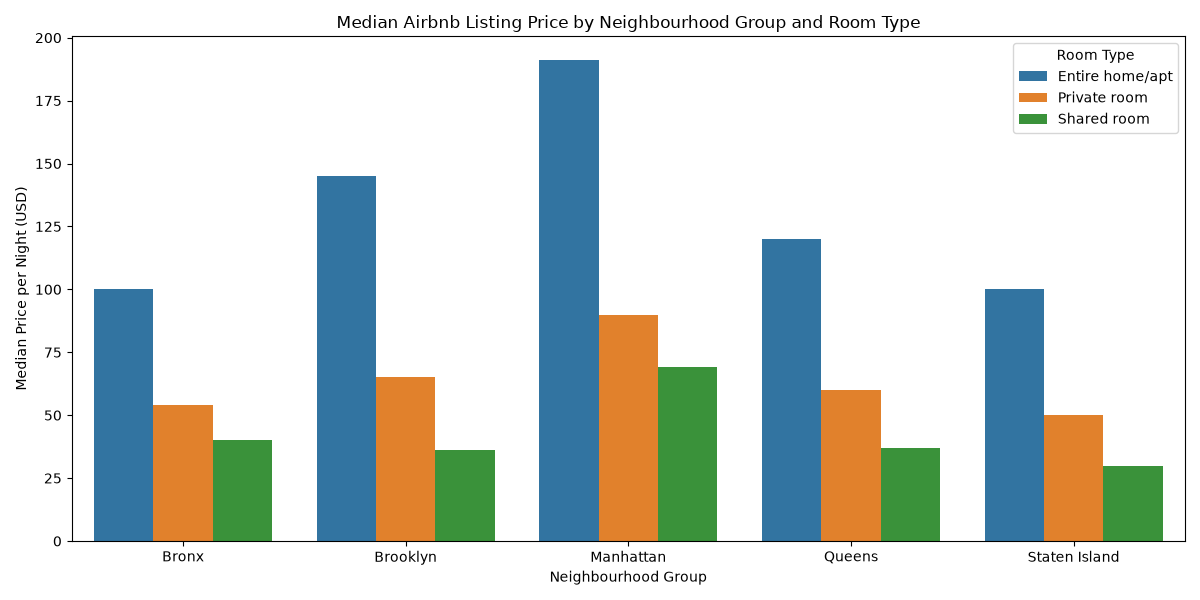
\includegraphics[width=\textwidth]
        {../figures/figure1_median_price.png}
    \caption{Median Airbnb listing price by neighbourhood group and room type.}
    \label{fig:median-price}
\end{figure}

\subsection{Price Distributions}

Figure~\ref{fig:price-distribution} shows that the distributions differ clearly
by room type. Entire homes and apartments have both the highest median and the
widest interquartile range. Private and shared rooms are concentrated at lower
prices, although both categories still contain relatively expensive listings.

All three distributions are right-skewed and contain many observations above
their upper box-plot whiskers. These observations are statistical outliers
under the box-plot convention but are not necessarily erroneous records. The
figure therefore supports retaining the observations while using median values
to describe typical prices.

\begin{figure}[H]
    \centering
    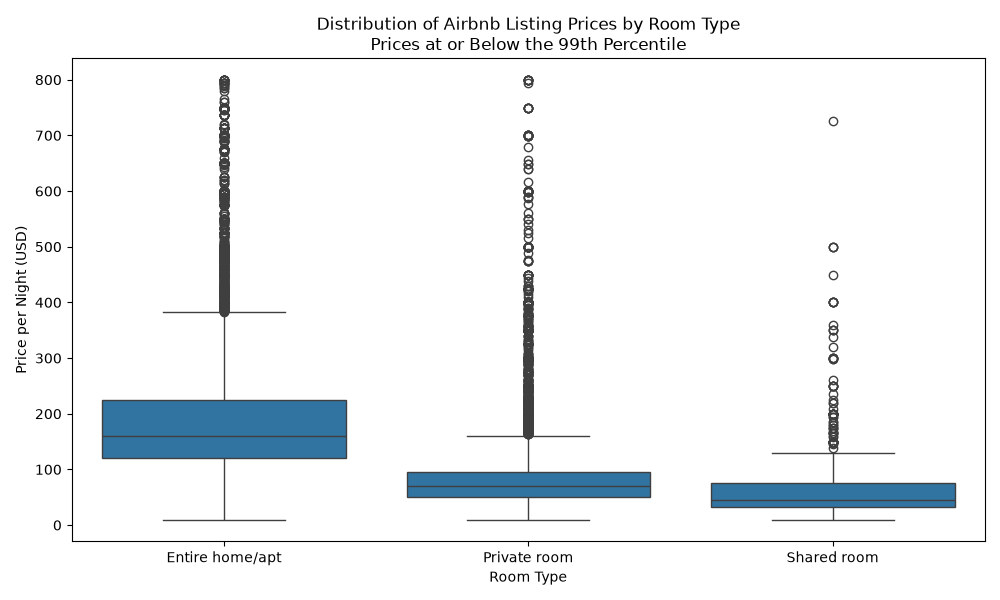
\includegraphics[width=0.9\textwidth]
        {../figures/figure2_price_distribution.png}
    \caption{Distribution of listing prices by room type for prices at or below
    the 99th percentile.}
    \label{fig:price-distribution}
\end{figure}

\subsection{Annual Availability}

Figure~\ref{fig:availability} shows substantial variation in median annual
availability. Staten Island has the highest typical availability for private
rooms, at approximately 280 days, and for entire homes and apartments, at
approximately 175 days. Manhattan and Brooklyn have much lower median
availability for these categories, generally below 50 days.

Shared rooms show a different pattern. Their median availability is relatively
high in Brooklyn and Queens but low in Staten Island. The results indicate that
availability patterns depend on the combination of neighbourhood group and
room type.

A total of 17,530 listings, or 35.86\% of the cleaned dataset, have zero
recorded availability. The proportion is highest in Brooklyn at 39.02\%,
followed by Manhattan at 37.40\%. Staten Island has the lowest proportion at
11.26\%.

\begin{figure}[H]
    \centering
    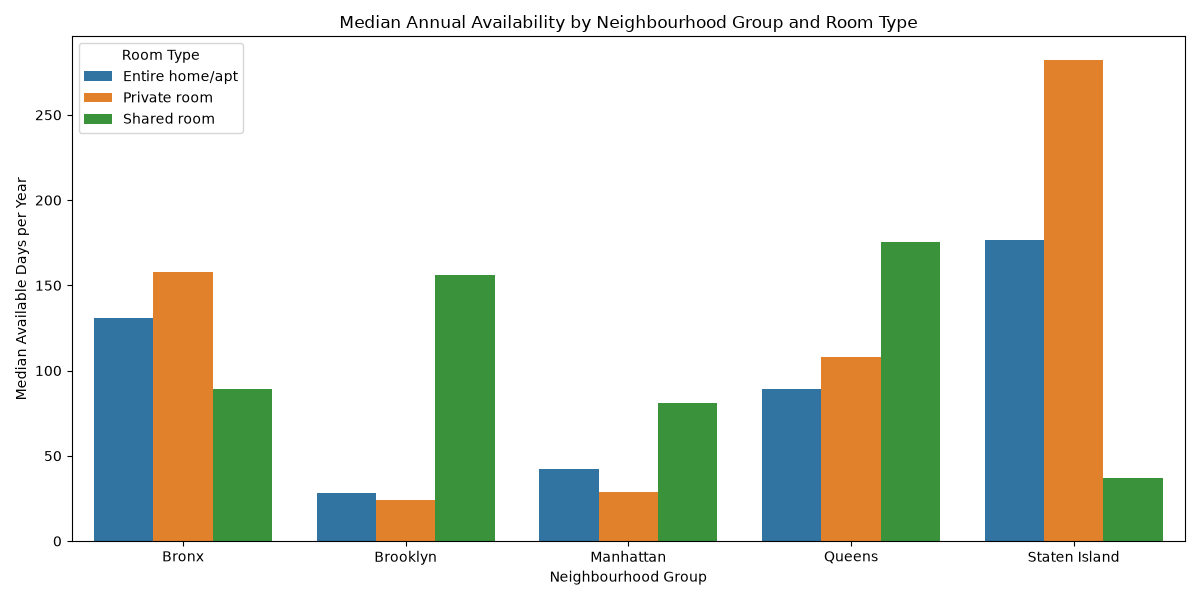
\includegraphics[width=\textwidth]
        {../figures/figure3_availability.png}
    \caption{Median annual availability by neighbourhood group and room type.}
    \label{fig:availability}
\end{figure}

\subsection{Numerical Correlations}

Most numerical variables have only weak linear relationships, as shown in
Figure~\ref{fig:correlation}. The strongest correlation is between
\texttt{number\_of\_reviews} and \texttt{reviews\_per\_month}, with a
coefficient of 0.59. This moderate positive association is expected because
both variables measure review activity.

A weaker but more substantively interesting relationship occurs between
\texttt{calculated\_host\_listings\_count} and
\texttt{availability\_365}, with a coefficient of 0.23. Listings associated
with hosts managing more properties tend to have slightly greater recorded
availability, but this relationship is weak and cannot establish causation.

Price has very weak correlations with all included numerical variables. Its
largest numerical correlation is only 0.08, with annual availability. The
grouped results therefore suggest that neighbourhood group and room type are
more informative for describing price differences than the numerical variables
included in the correlation analysis.

\begin{figure}[H]
    \centering
    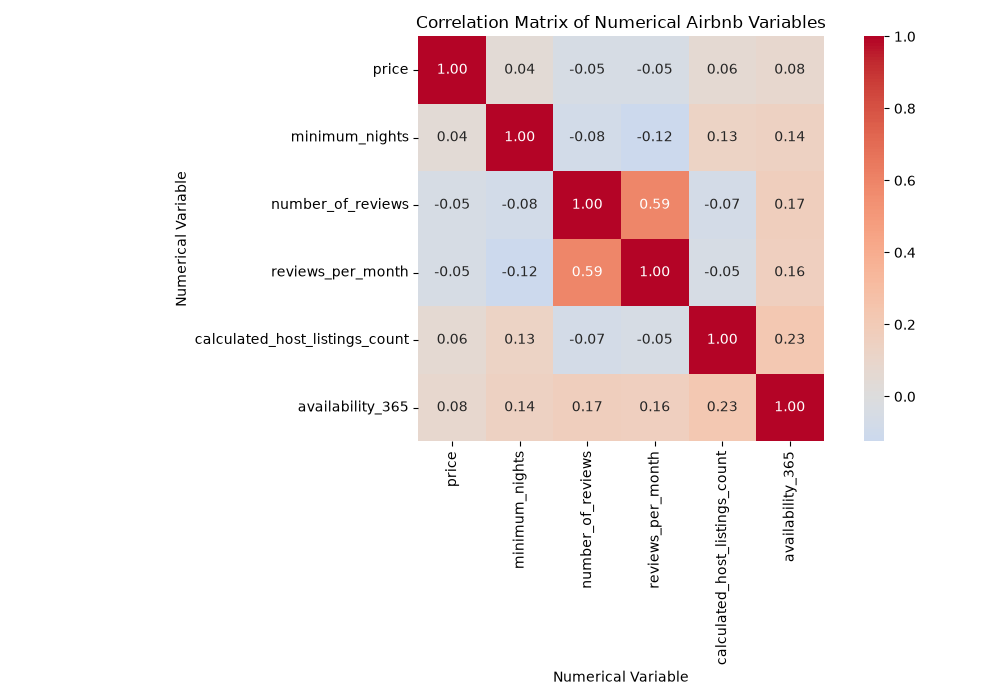
\includegraphics[width=0.82\textwidth]
        {../figures/figure4_correlation.png}
    \caption{Pearson correlation matrix for selected numerical variables.}
    \label{fig:correlation}
\end{figure}
